\section{Aplicación de ejemplo}

Para comprender mejor esta problemática veamos un ejemplo. Supongamos una simple
aplicación, donde los clientes de un banco pueden transferir dinero de
una cuenta a otra. Al realizar una transferencia, hay que extraer el monto
indicado de una cuenta, y depositarlo en otra. Estas dos
operaciones pueden tener errores, como por ejemplo, extraer un monto mayor al
saldo, o depositar una cantidad mayor a la máxima permitida. 
Un cliente no puede ver el saldo de las las cuentas que no sean de su propiedad.

La  figura \ref{example} muestra el diagrama de la aplicación de
ejemplo

	\begin{figure}[h]
		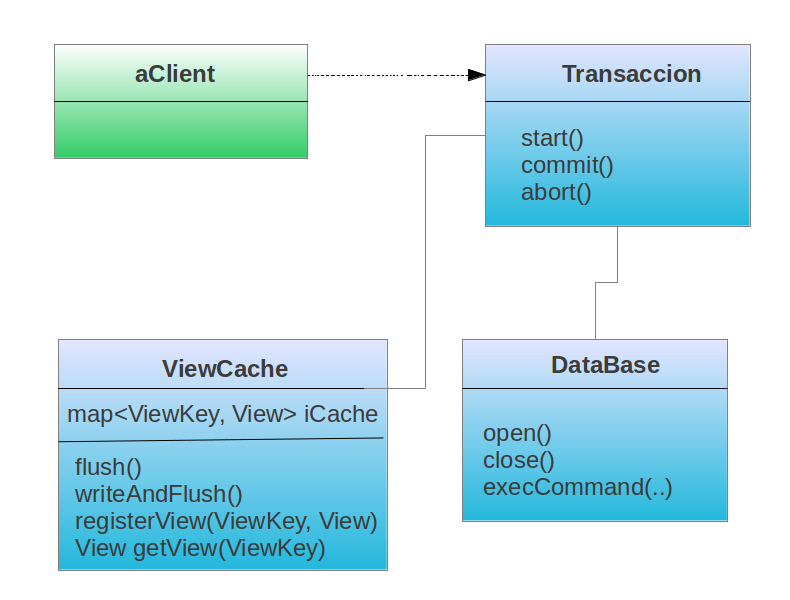
\includegraphics{img/objectTransaction}
		\caption{Diagrama UML de la aplicación de ejemplo}
		\label{example}
	\end{figure}	


El sistema me permite realizar múltiples transferencias a la vez y por ultimo
realizar la confirmación o la cancelación de todas ellas. También brinda la posibilidad
de realizar múltiples transacciones, por ejemplo, en la edición de un cliente,
se puede editar, eliminar o crear cuentas. A su vez se puede hacer una
transferencia a otra cuenta. En cada una de esas operaciones se esta
trabajando en dentro de una transacción. y las operaciones pueden ser
canceladas por unidad, es decir, se cancelan o se confirman por transacción.



\section{Nuestra herramienta: }

En esta sección se explica como se llevo a cabo la implementación de la solución
propuesta en la Sección \ref{sec:Solucion}, y cumpliendo el objetivo detallado
en la Sección \ref{sec:Objetivo}. Se desarrolló dos conceptos fundamentales
para con lo planteado. \emph{Pure Objects Observable} (POO)  para atacar a la
problemática de la observabilidad y \emph{Pure Object Transaction} (POT) para
atacar a la problemática transaccional.
	
	\subsection{Framework utilizado}  

	Se evaluaron dos frameworks para resolver nuestro problema. Uno es Javassist y
	el otro AspectJ. \cite{KiczalesHHKPG01}
	El criterio de evaluación que se utilizo fue el que tenga menor impacto para el
	programador que utilice el framework.

	\medskip 
	Aunque AspectJ es una herramienta de mas alto nivel en comparación con
	Javassist,  se eligió a  Javassist porque el agrega los aspectos al momento de
	la carga de la clase, es decir hay que utilizar un \emph{ClassLoader}
	específico, en cambio AspectJ agrega los aspectos al en tiempo de compilación,
	entonces el programador tienen que utilizar otro compilador para su código.

	\medskip 

	\subsection{Desarrollo de Aspect for Pure Objects}

	Ya que Javassist es muy de bajo nivel, y trabaja a nivel de \emph{bytecode},
	trabajar con el es complicado y el código se hace poco entendible. Por eso se
	desarrolló una herramienta llamada \emph{ Aspect for Pure Objects} (APO), que
	es una abstracción del Framework Javassist, que permite fácilmente configurar 
	aspectos, y aplicárselo a un grupo de objetos.

	\subsection{Aspecto Transaccional (POT)} 
		Basado en una implementación
		hecha por Nicolás Passerini y Javier Fernandes.
		 
		Donde intercepta todas las lecturas	y escrituras de los atributos de un
		objeto.	Insertando código al momento de la carga de la clase.
		Se remplaza el acceso al atributo, tanto de lectura como escritura, y se lo
		delega al administrador de las transacciones, donde se guarda la información
		en una estructura [Objeto, [Atributo, Valor]].
		
		\medskip
		
		El contexto de la transacción esta asociado a un solo \emph{tread}. Esto
		permite manejar la concurrencia en el acceso a la información de los objetos. 
		Soportando transacciones anidadas, donde cada transacción hija hereda el estado
		de su padre, y al momento de hacer el \emph{commit} en la sub-transacción, sus
		cambios son impactados en la transacción padre.
		Por esta forma de implementación, la identidad del objeto se mantiene, ya que
		el objeto no se modifica ni se clona, solo se cambia el acceso a sus
		atributos.
		
		Para agregarle este aspecto a una clase se utiliza la \emph{Annotation}
		\emph{Transactional }
				
		\begin{figure}[h]
				\begin{lstlisting} 
					@Transactional
					public class Client extends Entity {
					}
				\end{lstlisting}
			\caption{Ejemplo de uso del Aspecto Transaccional}
			\label{pot}
		\end{figure}  

	\subsection{ Aspecto Observable (POO)}
			
		En su implementación interna lo que hace el aspecto es agregar un \emph{field
		changeSupport} del tipo \emph{<<PropertySupport>>} al objeto que se va a
		convertir en Observable. Pero su implementación se obtiene del el archivo de
		configuración con la \emph{key: framework.aop.poo.changeSupport}.
		Luego se agrega métodos para completar su objetivo.
		El primero es el \emph{firePropertyChange} que es el que notifica a los
		Observadores que una propiedad ha cambiado.	Luego le agregamos
		\emph{addPropertyChangeListener} y \emph{removePropertyChangeListener} para
		poder agregar y remover Observadores para que escuchen sus cambios.
		
		Para agregarle este aspecto a una clase se utiliza la \emph{Annotation}
		\emph{Observable}
		
	\begin{figure}[h]
		\begin{lstlisting} 
			@Observable
			public class Client extends Entity {
			}
		\end{lstlisting}
		\caption{Ejemplo de uso del aspecto observable}
		\label{poo}
	\end{figure}  
		


\subsection{Integración de ambos aspectos } 
	Framework me permite poder tener uno u otro , o
	ambos aspecto. Se puede poner los dos \emph{Annotation} \emph{Observable} y
	\emph{Transactional} como vimos previamente, o ponerle uno solo. 
	
	\begin{figure}[h]
		\begin{lstlisting} 
			@TransactionalAndObservable
			public class Client extends Entity {
			}
		\end{lstlisting}
		\caption{integración de ambos aspectos}
		\label{TandO}
	\end{figure}  
	
	
	
\subsection{Integración de aspectos con el Arena}
	En Arena se integró los dos aspectos, el Observable y el transaccional, con el
	fin de que los objetos de dominio sean puros, y que no tengan la noción de
	eventos, ni transacciones, y así poder bindearlos con los componentes de de la
	interfaz gráfica. Y al cancelar la edición poder revertir los cambios
	transparéntenme.
	
	Para ello se tubo que asociar una transacción con una ventana, en el caso mas
	especifico con la clase \emph{TransactionalDialog}. A su vez también tenemos
	vinculado los eventos del dominio junto con la ventana y la transacción.
	Se implemento tres niveles de aislamiento de los eventos,  \emph{Fire All},
	\emph{Fire Committed} y \emph{Fire olnly in my transaction};
	
	\begin{description}
		\item[\emph{Fire All}] Todos los eventos disparados por el dominio son
		escuchados, sin importar si están en una transacción.
	
		\item[\emph{Fire Committed}] Solo se escucha los eventos de las transacciones
			comiteadas
		
		\item[\emph{Fire olnly in my transaction}] solo se escucha los eventos que
			ocurren dentro de su translación.
	
	 \end{description}
	 
	 \medskip
	 

	
	\subsection{Otras mejoras al Arena}
	La integración se realizo con el lenguaje de programación Scala
	\cite{ref}. Para llevar al cabo la integración se agregó algunas
	mejoras en el Arena. 
	Algunas mejoras fueron:
	\begin{description}
	  \item[Monitor de Transacciones]
		 Con arena también se desarrolló un \emph{Monitor de Transacciones}, que 
		 muestra el estado actual de la transacción, incluyendo las transacciones
		 anidadas. Mostrando los objetos afectados por la transacción y los
		 atributos se modificaron.
	  \item[Nuevos componentes] Se Implementaron algunas estructuras visuales como
	  Arboles y Listas.
	  \item[Bindinds Anidados] Se implemento bindings para las propiedades
	  anidadas de los objetos.
	\end{description}
